\documentclass[conference]{IEEEtran}
\IEEEoverridecommandlockouts

\usepackage{cite}
\usepackage{amsmath,amssymb,amsfonts}
\usepackage{algorithmic}
\usepackage{graphicx}
\usepackage{textcomp}
\usepackage{xcolor}
\usepackage{booktabs}
\usepackage{tikz}
\usetikzlibrary{arrows.meta,positioning,fit,backgrounds}
\usepackage{url}
\usepackage[hidelinks]{hyperref}

\newcommand{\tbd}[1]{\textcolor{red}{[TBD: #1]}}

\begin{document}

\title{An Open Streaming Validation Platform for\\Reconfigurable Holographic Surface Beamforming}

\author{
\IEEEauthorblockN{Author Name}
\IEEEauthorblockA{Affiliation\\City, Country\\email@example.org}
}

\maketitle

\begin{abstract}
Reconfigurable holographic surfaces (RHS) promise compact, low-cost
beamforming, but comparing learned beamformers with classical optimisation is
hindered by fragmented data pipelines, ad-hoc metrics, and the absence of a
shared hardware--software contract. This paper presents an open, containerised
validation platform that streams RHS configurations from a simulator, an
STM32/ESP32 gateway, or an HDMI capture path into a framed, ACK-driven
protocol. A FastAPI inference service evaluates GP ground truth and two learned
beamformers (a hand-designed hybrid model and a NAS-discovered model), while a
provenance layer records every hop in MongoDB and Redis. The platform exposes a
retro monochrome operator console and a browsable artifact registry. We describe
the architecture, the frame format and handshake, the eigen-spectrum-based
model-selection policy, and a reproducible deployment on commodity hardware.
\end{abstract}

\begin{IEEEkeywords}
reconfigurable holographic surfaces, beamforming, validation platform,
streaming, neural architecture search, reproducible research
\end{IEEEkeywords}

\section{Introduction}
\IEEEPARstart{R}{econfigurable} holographic surfaces (RHS) implement
beamforming through arrays of sub-wavelength radiating elements whose
excitation is tuned in amplitude and phase. Classical gradient-based
optimisation provides a strong reference, but its cost grows with the number of
elements and iterations, motivating learned beamformers that amortise inference.
Comparing such models is difficult in practice: datasets, normalisation,
evaluation splits, and hardware transports are usually re-implemented per
study, and reported gains are rarely traceable end to end.

This paper addresses the reproducibility gap with a validation platform rather
than another beamformer. The contributions are:
\begin{itemize}
  \item a five-service deployment (frontend, backend, inference, MongoDB,
        Redis) with a stable HTTP contract and a retro operator UI;
  \item a compact binary frame format with CRC32 and a four-step
        request/acknowledge handshake that is shared by Python services, an
        STM32 firmware reference, and an ESP32 Wi-Fi bridge;
  \item a model-selection policy that combines eigen-spectrum agreement,
        beamforming cosine similarity, rate error, and latency;
  \item a provenance model that records source, travel, destination, and
        validation hops for every published sample.
\end{itemize}

\section{Related Work}
\tbd{Position against RHS beamforming, learned beamforming, and reproducible
testbeds.}

\section{System Architecture}
Figure~\ref{fig:arch} shows the deployment. The \emph{frontend} is an nginx
reverse proxy serving a server-rendered monochrome UI. The \emph{backend}
validates requests, performs the frame handshake, calls the inference service,
computes the GP--DL difference report, and persists provenance. The
\emph{inference} service loads the GP fixture and both learned checkpoints,
calibrates JEV profiles, and answers prediction and switching requests.
MongoDB stores durable documents; Redis stores ACK state, streams, and the
active-model cache.

\begin{figure}[t]
\centering
\resizebox{\columnwidth}{!}{%
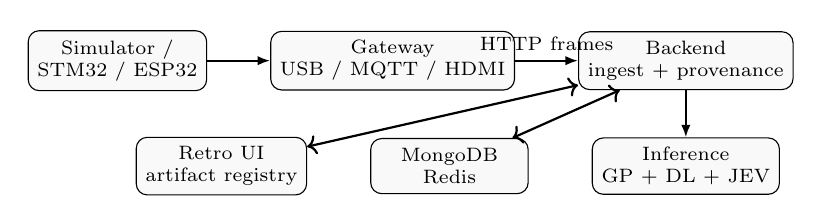
\begin{tikzpicture}[
  node distance=6mm and 8mm,
  box/.style={draw, rounded corners, align=center, font=\scriptsize,
              minimum height=7mm, minimum width=20mm, fill=gray!5},
  arr/.style={-{Latex[length=1.6mm]}, thick}
]
\node[box] (sim) {Simulator /\\STM32 / ESP32};
\node[box, right=of sim] (gw) {Gateway\\USB / MQTT / HDMI};
\node[box, right=of gw] (be) {Backend\\ingest + provenance};
\node[box, below=of be] (inf) {Inference\\GP + DL + JEV};
\node[box, left=of inf] (db) {MongoDB\\Redis};
\node[box, left=of db] (fe) {Retro UI\\artifact registry};
\draw[arr] (sim) -- (gw);
\draw[arr] (gw) -- node[above, font=\scriptsize]{HTTP frames} (be);
\draw[arr] (be) -- (inf);
\draw[arr, <->] (be) -- (db);
\draw[arr, <->] (fe) -- (be);
\end{tikzpicture}%
}
\caption{Five-container validation platform. The gateway is optional for
simulator-only runs.}
\label{fig:arch}
\end{figure}

\section{Streaming Protocol}
\subsection{Frame format}
Each frame carries a four-byte magic, a version byte, a message type, a 32-bit
sequence number, a 32-bit payload length, the JSON payload, and a CRC32 over all
preceding bytes. The CRC uses the IEEE 802.3 polynomial, matching
\texttt{zlib.crc32} and the STM32 implementation bit for bit.
Table~\ref{tab:frames} lists the message types.

\begin{table}[t]
\centering
\caption{Protocol message types.}
\label{tab:frames}
\begin{tabular}{@{}cll@{}}
\toprule
ID & Type & Role \\
\midrule
1 & \texttt{DATA\_REQ} & host announces a sample \\
2 & \texttt{RECV\_OK} & device accepts, returns JEV decision \\
3 & \texttt{DATA\_ACK} & host confirms receipt \\
4 & \texttt{JEV\_DECISION} & optional decision notification \\
5 & \texttt{MODEL\_SWITCH} & request a different checkpoint \\
6 & \texttt{RESULT} & diff report and artifact URLs \\
7 & \texttt{ERROR} & recoverable failure \\
\bottomrule
\end{tabular}
\end{table}

\subsection{Handshake}
The host sends \texttt{DATA\_REQ} with a sample identifier. The backend records
the pending sample, asks the inference service for a JEV decision, and returns
\texttt{RECV\_OK} with the selected model and confidence. After the host sends
\texttt{DATA\_ACK}, the backend publishes the sample, computes the GP--DL
difference, and returns \texttt{RESULT}. State is mirrored in Redis so a
gateway can retry or resume after a disconnect.

\section{Model Selection}
For a configuration with known GP ground truth, the probe signature is the
log-compressed top-$k$ softmax of the GP beamforming Gram spectrum. Each
candidate model is executed once, and its own signature is compared with the
probe. The score combines spectral distance, beamforming cosine similarity, rate
error, and normalised inference latency:
\begin{multline}
s_m = \lambda_s \lVert p - q_m \rVert_1
      + (1-\cos(\mathbf{M}_{\mathrm{GP}},\mathbf{M}_m)) \\
      + 0.05\frac{|r_m-r_{\mathrm{GP}}|}{\sigma_r}
      + \lambda_\ell \frac{\ell_m}{\max_j \ell_j}.
\end{multline}
Defaults are $\lambda_s=0.2$ and $\lambda_\ell=0.05$. The GP model is retained
as an explicit reference but excluded from automatic selection, so the platform
always reports a learned beamformer and its distance to the oracle.

\section{Deployment and Reproducibility}
The stack is described by a single Compose file and builds from CPU-only
Python~3.12 images. Host ports are remapped to avoid collisions with an
existing edge stack. All data, checkpoints, source, and paper artifacts are
mounted read-only; the only writable state is MongoDB and Redis. Table~\ref{tab:deploy}
summarises the services.

\begin{table}[t]
\centering
\caption{Service deployment.}
\label{tab:deploy}
\begin{tabular}{@{}llll@{}}
\toprule
Service & Image & Port & State \\
\midrule
Frontend & nginx 1.27 & 8088 & stateless \\
Backend & Python 3.12 & 8090 & Mongo/Redis \\
Inference & Python 3.12 + Torch & 8091 & read-only \\
MongoDB & mongo 7 & 27018 & volume \\
Redis & redis 7 & 6380 & volume \\
\bottomrule
\end{tabular}
\end{table}

\section{Evaluation}
\tbd{Report end-to-end latency, ingestion throughput, handshake reliability,
and a comparison of hybrid vs NAS-selected beamformers over the held-out split.
Current model-card values: hybrid rate $R^2=0.8044$, $M$ cosine $0.7772$;
NAS-selected $R^2=0.7877$, $M$ cosine $0.7688$; 997{,}825 parameters.}

\section{Discussion and Limitations}
The platform deliberately separates physics from architecture: the shared
\texttt{rhs\_beamforming} package owns geometry, channel, MMSE, rate, and
constraints, while models are interchangeable checkpoints. The current GP path
uses dataset ground truth rather than solving the GP program online; extending
the inference service with a live solver is future work. Hardware validation is
simulator-first; USB capture, MQTT, and v4l2 paths are implemented but require
attached devices.

\section{Conclusion}
We presented an open streaming validation platform for RHS beamforming that
couples a reproducible container deployment, a firmware-compatible frame
protocol, provenance tracking, and a transparent model-selection policy. The
platform turns a collection of checkpoints into an auditable, end-to-end
comparison against the GP reference.

\begin{thebibliography}{00}
\bibitem{ref1} \tbd{Add RHS and learned beamforming references.}
\bibitem{ref2} \tbd{Add reproducible testbed references.}
\end{thebibliography}

\end{document}
